\documentclass[10pt]{report}

  \usepackage{multicol}
\usepackage[a4paper, margin=0.5in]{geometry}
\usepackage{amsmath, amssymb, graphicx, xcolor, float, hyperref, wrapfig, hyperref, setspace, tikz}
\usetikzlibrary{arrows.meta, positioning, shapes.geometric}
% Styles
\tikzset{
  box/.style = {rectangle, draw=black, rounded corners, minimum width=4.5cm, minimum height=1.1cm, align=left, font=\small, inner sep=6pt},
  arr/.style = {-latex}
}

\begin{document}
  \begin{titlepage}
    \centering
    \textit{\LARGE Concept Note}\\
    \vspace{0.5cm}
    \textbf{\huge Amateur Experimental Rocketry} \\
    \vspace{0.5in}
    \textit{\large (This project is a continuation of Summer Internship 2025 Synopsis titled)}\\
    \vspace{0.1cm}
    \textbf{\large Design and Simulation of a CanSat-Based Hobby Rocket \\ Using OpenRocket and EasyEDA}\\
    \vspace{0.5in}
    \textbf{\large Project Title:} \\
    \vspace{0.5cm}
    \textbf{\Large Design and Development of a Low-Powered \\ Solid Propellant Model Rocket with Thrust Vector Control} \\
    \vspace{0.2cm}
    \textit{An Undergraduate Initiative in Model Rocketry and Propulsion Studies}\\
    \vspace{0.5cm}
  \begin{figure}[h!]
    \centering
    \begin{minipage}[t]{0.1\textwidth}
        \centering
        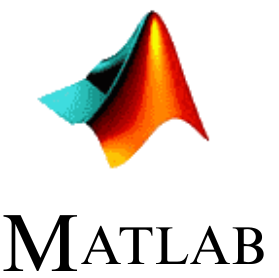
\includegraphics[width=\textwidth]{matlab.png}
    \end{minipage}%
        \hspace{0.8in}
    \begin{minipage}[t]{0.1\textwidth}
        \centering
        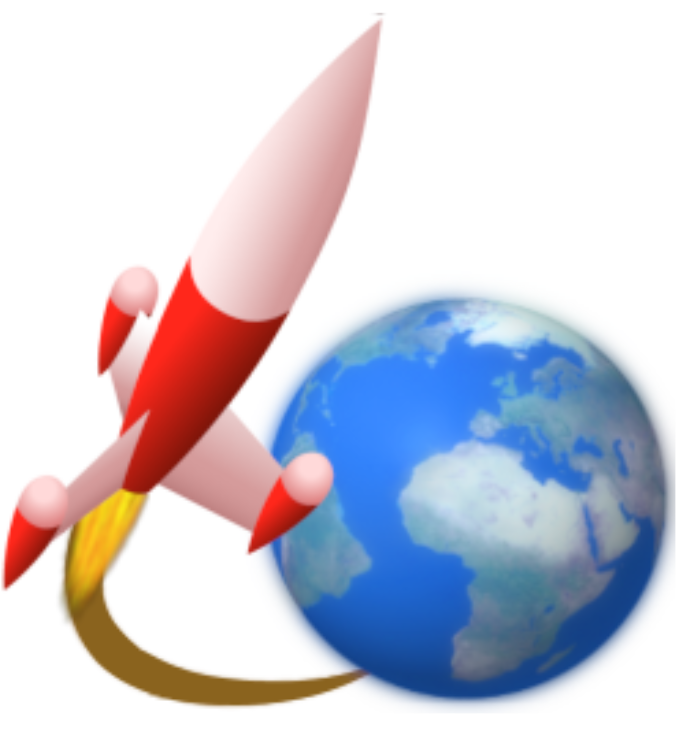
\includegraphics[width=\textwidth]{openrocket.png}
    \end{minipage}%
\end{figure}
    \vspace{0.5in}
    {\large Contributors:} \\
    \textbf{\large Anirban Das [23EC009]} -- \href{mailto:anirban.das_btech23@gsv.ac.in}{\textit{anirban.das\_btech23@gsv.ac.in}} \\ 
    \textbf{\large Aman Chowdhary [23ME101]} -- \href{mailto:aman.chowdhary_btech23@gsv.ac.in}{\textit{aman.chowdhary\_btech23@gsv.ac.in}}\\
    \vspace{0.5in} 
    \textit{\large submitted to }\\
    \vspace{0.2in} 
    \textbf{\Large Dr. V. Chintala} \\
    {\large [ Registrar \& Head ]} \\ \textbf{\large [ Airbus Center of Excellence ]} \\
    \vspace{0.1in}
    
\includegraphics[width=0.25\textwidth]{gsv_logo.png}\\
    \vspace{0.5cm} 
    \textbf{\large GATI SHAKTI VISHWAVIDYALAYA} \\
    {\large (A Central University under Ministry of Railways, Govt. of India) \\ Vadodara, Gujarat \\ 390004} \\

  \end{titlepage}
  \newpage 

  \begin{center}
    \textbf{\LARGE Statement of Purpose}
    \addcontentsline{toc}{section}{\large i. \textbf{Statement of Purpose}}
  \end{center}

  For about a year now, we have been exploring the field of rocketry and propulsion systems. The idea of designing, building, and launching rockets has always intrigued me, and we've spent a significant amount of time researching and learning about the various aspects of rocketry. This project aims to provide hands-on experience in the field of rocketry, allowing us to apply theoretical knowledge to practical applications. The project will involve the design, development and testing of a low-powered solid propellant model rocket. \\

  This project is significant because it will provide me with a deeper understanding of the principles of rocketry, propulsion systems, and aerodynamics. It will also help me develop skills in areas such as CAD design, simulation, and testing. The project will be divided into several phases, each focusing on a specific aspect of the rocket's design and development. The phases will include baseline rocket validation, recovery system integration, avionics and telemetry deployment, and thrust vector control implementation. Each phase will involve a series of tests and evaluations to ensure that the rocket meets the required performance and is safe to launch.
  \\

  There is another motivation for this initiative. Currently, India is lacking behind in terms of reusable booster technology. On October 13, 2024, SpaceX did the impossible by catching one of their super-heavy boosters -- a marvel of aerospace engineering. The precision and accuracy of that maneuver was so impressive and complex, that till now, only a few other countries have been able to achieve it, and India is not one of them, \textbf{\textit{yet!}}. Thru this project, I would explore ways to develop such tech indigenously and at affordable prices.

  \newpage 
  \begin{center}
    \textbf{\LARGE Acknowledgements}
    \addcontentsline{toc}{section}{\large ii. \textbf{Acknowledgements}}
  \end{center}

    In the completion of this project, I would like to express my deepest gratitude to my professors for their invaluable guidance and support. Their expertise and encouragement have been instrumental in the successful completion of this work. \\

I am especially grateful to \textbf{Dr. V. Chintala} for his guidance in directing this project. his expertise on fuel chemistry have shaped the overall outcome of this project in ways I cannot pen down into words. Their insights have greatly contributed to my understanding and the direction of this project. \\

I am also grateful to \textbf{Mr. Munnavar Pathan} \& \textbf{Mr. Sachin} for their continual support and for providing the resources needed to complete this project.  \\

Thank you all for your patience, motivation, and immense knowledge. This project would not have been possible without your support.
  
 % ========================= [CONTENTS] ========================
  \begin{spacing}{2}
    \tableofcontents
  \end{spacing}

  \newpage
\begin{center}
    \textbf{\LARGE PHASE - I} \\
    \vspace{0.2cm}
    \textbf{\Large Baseline Rocket Validation (Propellant + Stability Test)}
  \end{center}
  \addcontentsline{toc}{section}{\large 1. \textbf{PHASE - I :} Baseline Rocket Validation (Propellant + Stability Test)}

  \begin{multicols}{2}
      
  \section*{OBJECTIVE:}  \textit{Verify aerodynamic stability and motor performance using KNSu family propellant.} \\
  The main objective of this phase per-se is to validate the baseline design of the model rocket, ensuring that it meets the necessary performance and safety criteria. This phase will involve a series of tests and evaluations to assess the rocket's aerodynamic stability and motor performance. The primary focus will be on using KNSu (Potassium Nitrate and Sugar) family propellant, which is a common choice for amateur rocketry due to its ease of preparation and relatively safe handling characteristics. \\

  We are not incorporating any electronics in this phase, as the primary goal is to validate the basic design and performance of the rocket. By focusing on the fundamental aspects of rocketry, I can ensure that the rocket is stable and performs as expected before adding more complex systems such as avionics and thrust vector control. This approach allows for a more systematic development process, reducing the risk of complications arising from integrating multiple systems at once. \\

  \section*{DESIGN:} \textit{Airframe geometry, CP/CG targets, fins, mass-budget}\\
  We have tried to incorporate the airfoil shape in the nosecone design to minimize drag and improve aerodynamic efficiency. The nosecone will be designed using CAD software, ensuring a smooth and streamlined shape that reduces air resistance during flight. The center of pressure (CP) and center of gravity (CG) targets will be carefully calculated to ensure that the rocket remains stable during flight. The CP will be positioned behind the CG to provide a positive stability margin, which is essential for maintaining a stable flight trajectory. \\

  A more detailed design schematic has been attached in the next pages. \\

  \section*{ MATERIALS \& TOOLS:} \textit{Body-Tube (UPVC), Nosecone (PLA 100\% infill), custom motor casing (PLA (100\% infill)), static test stand.}\\
  We have chosen to use a cheap PVC pipe as our body tube. This is economically viable, as-well as lightweight -- proving the best choice for rapid prototyping. The nosecone, motor casing and fin structures will be 3D printed using PLA material. The motor casing will be custom designed to fit the KNSu propellant grains, ensuring optimal performance and safety during the rocket's flight. The fins will be designed to provide the necessary stability during flight, with careful consideration given to their size, shape, and placement on the rocket. The overall design of the rocket will be optimized for aerodynamic efficiency, with a focus on achieving a stable flight trajectory and maximizing altitude. \\

  \section*{TESTS:}  \textit{Static motor firing (bench), glide tests, Drop Test, CP/CG alignment - horizontal suspension.} \\
  The static tests are important to validate the propellant grain density and homogenity of the grain structure. To achieve longer burn-time and slower burn rates, we are using \textbf{Sorbitol} as a replacement to Sucrose. \\

  To ensure that is grain is safe and ignites safely, \textbf{\textit{special care must be taken to ensure that bubbles are not formed during propellant curing.}} The air bubbles formed due to uneven setting of the propellant, can form un-even combustion chambers and result in explosion of the motor casing. \\

  To avoid this,  vacuum chambers are used to degas the propellant mixture before pouring it into the motor casing. But since we do not have such equipment, we shall just ensure that the \textit{sorbital-KNSU} paste is evenly settled into the casing. \\

  \section*{SUCCESS CRITERIA:}  \textit{stable flight trajectory, recovery of motor casing, measured stability margin $\geq$ 1 cal, apogee $\geq$ 100m.} \\
  This phase will be considered successful if the rocket demonstrates a stable flight trajectory, with a measured stability margin of at least 1 caliber. The motor casing should be recovered intact after the flight, indicating that the propellant performed as expected and that the rocket's design is robust enough to withstand the stresses of launch and recovery. Additionally, the rocket should reach an apogee of at least 100 meters, demonstrating that the motor provided sufficient thrust to achieve a significant altitude. \\

  \noindent \textbf{\large RISKS \& MITIGATION:}\\  \textit{propellant handling, fire extinguisher, blast shielding, remote igniter} \\
  The risks and mitigation strategies for this phase include: \\
\begin{itemize}
\item Propellant Handling: Proper safety protocols will be followed when handling the KNSu propellant, including wearing protective gear and working in a well-ventilated area. \\
  \item Fire Extinguisher: A fire extinguisher will be kept on hand during all testing activities to quickly address any potential fires that may arise. \\
  \item Blast Shielding: A blast shield will be used during static motor firing tests to protect against any potential explosions or debris. \\
 
\end{itemize}

  \end{multicols}
\noindent \textbf{IMPLEMENTATION FLOW:} \\
\vspace{0.5cm}

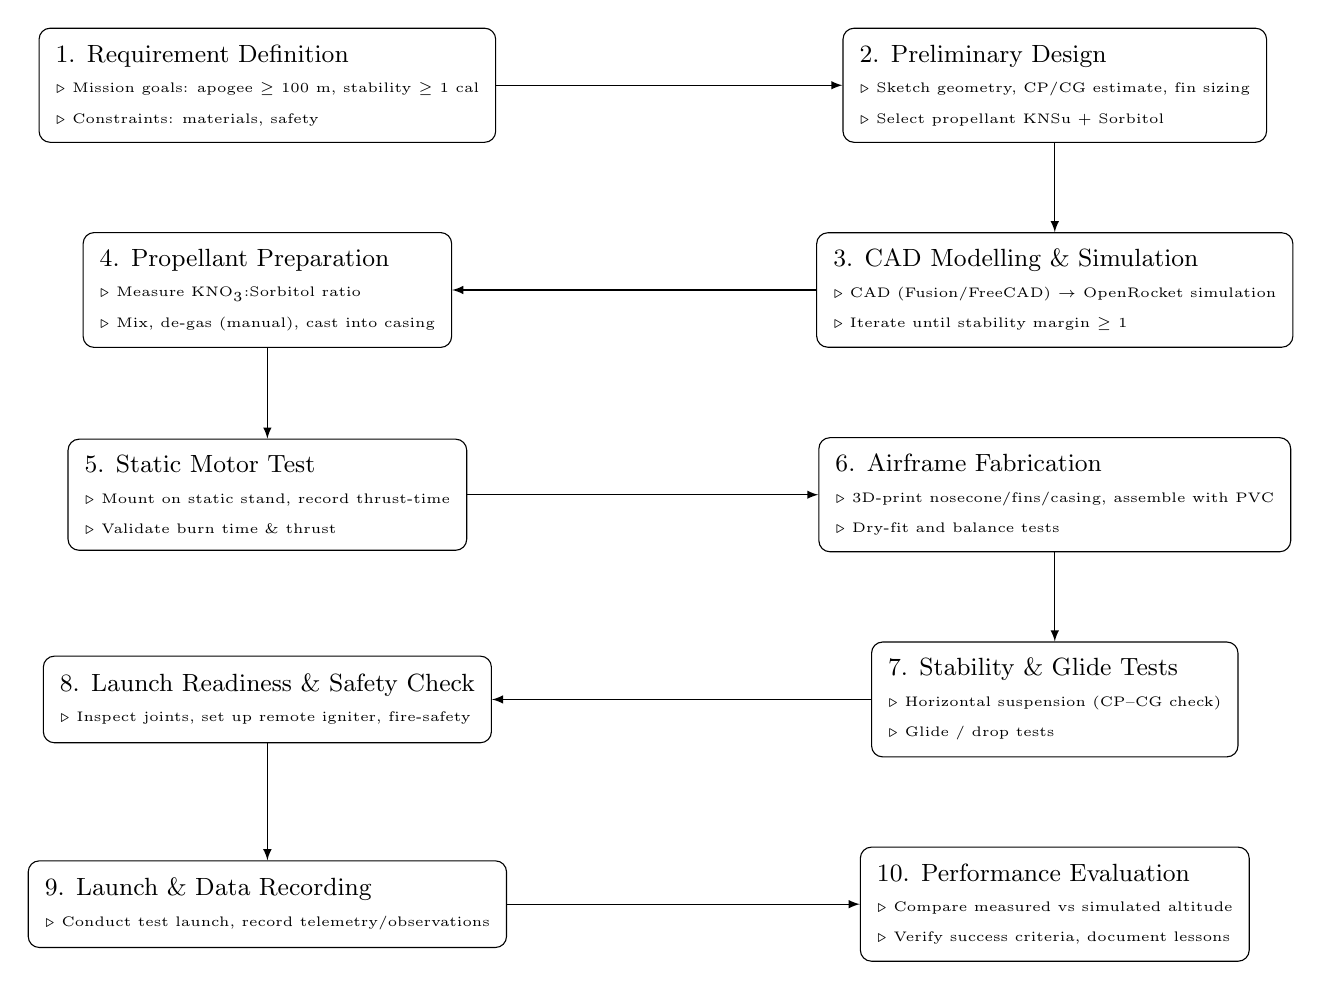
\begin{tikzpicture}[node distance=1.2cm and 1.0cm]

% Row 1 (left -> right)
\node[box] (n1)  at (0,0)   {1. Requirement Definition\\\tiny$\triangleright$ Mission goals: apogee $\geq$ 100 m, stability $\geq$ 1 cal\\\tiny$\triangleright$ Constraints: materials, safety};
\node[box] (n2)  at (10,0)   {2. Preliminary Design\\\tiny$\triangleright$ Sketch geometry, CP/CG estimate, fin sizing\\\tiny$\triangleright$ Select propellant KNSu + Sorbitol};

% Down from row1 end to row2 start
\node[box] (n3)  at (10,-2.6)  {3. CAD Modelling \& Simulation\\\tiny$\triangleright$ CAD (Fusion/FreeCAD) $\rightarrow$ OpenRocket simulation\\\tiny$\triangleright$ Iterate until stability margin $\geq$ 1};

\node[box] (n4)  at (0,-2.6){4. Propellant Preparation\\\tiny$\triangleright$ Measure KNO$_3$:Sorbitol ratio\\\tiny$\triangleright$ Mix, de-gas (manual), cast into casing};


\node[box] (n5)  at (0,-5.2){5. Static Motor Test\\\tiny$\triangleright$ Mount on static stand, record thrust-time\\\tiny$\triangleright$ Validate burn time \& thrust};
\node[box] (n6)  at (10,-5.2){6. Airframe Fabrication\\\tiny$\triangleright$ 3D-print nosecone/fins/casing, assemble with PVC\\\tiny$\triangleright$ Dry-fit and balance tests};

% Down to row3 (left->right)
\node[box] (n7)  at (10,-7.8){7. Stability \& Glide Tests\\\tiny$\triangleright$ Horizontal suspension (CP–CG check)\\\tiny$\triangleright$ Glide / drop tests};
\node[box] (n8)  at (0,-7.8){8. Launch Readiness \& Safety Check\\\tiny$\triangleright$ Inspect joints, set up remote igniter, fire-safety};

\node[box] (n9)  at (0,-10.4){9. Launch \& Data Recording\\\tiny$\triangleright$ Conduct test launch, record telemetry/observations};
% Final node (performance evaluation) centered below row3
\node[box] (n10) at (10,-10.4){10. Performance Evaluation\\\tiny$\triangleright$ Compare measured vs simulated altitude\\\tiny$\triangleright$ Verify success criteria, document lessons};

% Arrows: row1 left->right

% ----- CLEANED ARROWS -----
% Row1: left → right
\draw[arr] (n1.east) |- (n2.west);

% Down from row1 end to row2 start
\draw[arr] (n2.south) -| (n3.north);

% Row2: right → left
\draw[arr] (n3.west) |-  (n4.east);

% Down from row2 start to row3 start
\draw[arr] (n4.south) -| (n5.north);

% Row3: left → right
\draw[arr] (n5.east) |- (n6.west);

% Down from row3 end to row4 end
\draw[arr] (n6.south) -| (n7.north);

% Row4: right → left
\draw[arr] (n7.west) |- (n8.east);

% Down from row4 start to row5 start
\draw[arr] (n8.south) -| (n9.north);

% Row5: left → right
\draw[arr] (n9.east) |- (n10.west);


% Optional small captions (tiny numbers near nodes already inside)
% (If you want arrows with labels like "iterate" or "verify", add node[midway,above]{text} to each \draw)

\end{tikzpicture}

\newpage 
\begin{multicols*}{2}[
  \begin{center}
    \section*{SOLID MOTOR CASTING}
    \textbf{"Combustion is the marriage of hydrocarbons and oxygen"} \\
    \hfill  \textit{ -- Dr. V. Chintala}
  \end{center} ]
\subsection*{Propulsion Chemistry}
  Combustion is the fusion of an oxidizer and a fuel. For this project, we're initially going with the most common type of fuel for amateur hobby rocketry -- \textbf{KNSu (Potassium Nitrate + Sugar)}. 
  \[ \boldsymbol{\underbrace{KNO_3}_{65 \%} \; + \; \underbrace{C_{12} H_{22} O_{11}}_{35 \%}} \]

  \noindent The balanced stoichiometric equation is below:
  \[ C_{12}H_{22}O_{11} + 6 KNO_3 \rightarrow \underset{\textbf{potash}}{3K_2CO_3} + 3CO_2+11H_2O+6N_2 \] 

  \noindent A few drawbacks of using sucrose here is as follows:
  \begin{enumerate}
    \item Among all the by-products of the above reaction, one that stands out is $\; K_2 CO_3\;$, commonly knwon as \textbf{potash}. Potash is a solid residue that can accumulate inside the motor casing after combustion. Over time, this buildup can affect the performance of the rocket motor, potentially leading to reduced thrust and efficiency in subsequent launches. 
    \item  Water is used to dissolve the powders, but removing water later becomes an issue. Too much water can lead to incomplete combustion, while too little can make the mixture difficult to work with.
  \end{enumerate}

  We're working with a pressure engine, and hence, we would need to generate huge amounts of gase in a short span of time. To achieve this, we need to ensure that the burn rate of the propellant is sufficiently high. One way to increase the burn rate is by modifying the fuel component of the KNSu mixture. \\ 


  
    \subsection*{\small Results and Observations:}
  We performed a couple of mock tests with the Sugar+ $KNO_3$ configuration, and here's what we got: \\

  \noindent \textbf{Thrust v/s Time: } \\

    \noindent 1. Static Fire \#1 
      \begin{center}
          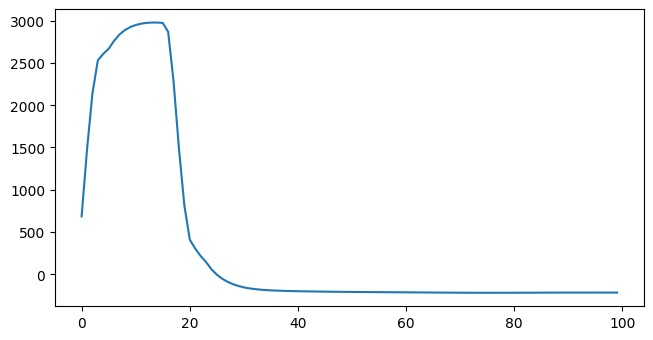
\includegraphics[width=0.4\textwidth]{sf_1.jpeg}
      \end{center} 
      We got about \textbf{30N} of thrust for about \textbf{2.5s} of burn time. The thrust curve was very spiky, which is a common issue with KNSu propellant due to its inconsistent burn characteristics. The peak thrust was around 30N, but it fluctuated significantly throughout the burn, indicating an unstable combustion process. \\ 
      \begin{figure}[H]
        \centering
        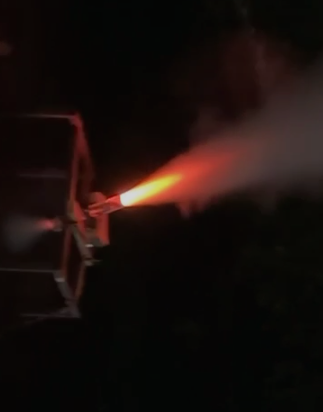
\includegraphics[width=0.25\textwidth, angle=90]{thrust_1.png}
        \caption{\small Static Fire \#1}
      \end{figure}

    \noindent 2. Static Fire \#2 \\
      \begin{wrapfigure}{l}{0.1\textwidth}
    \centering
      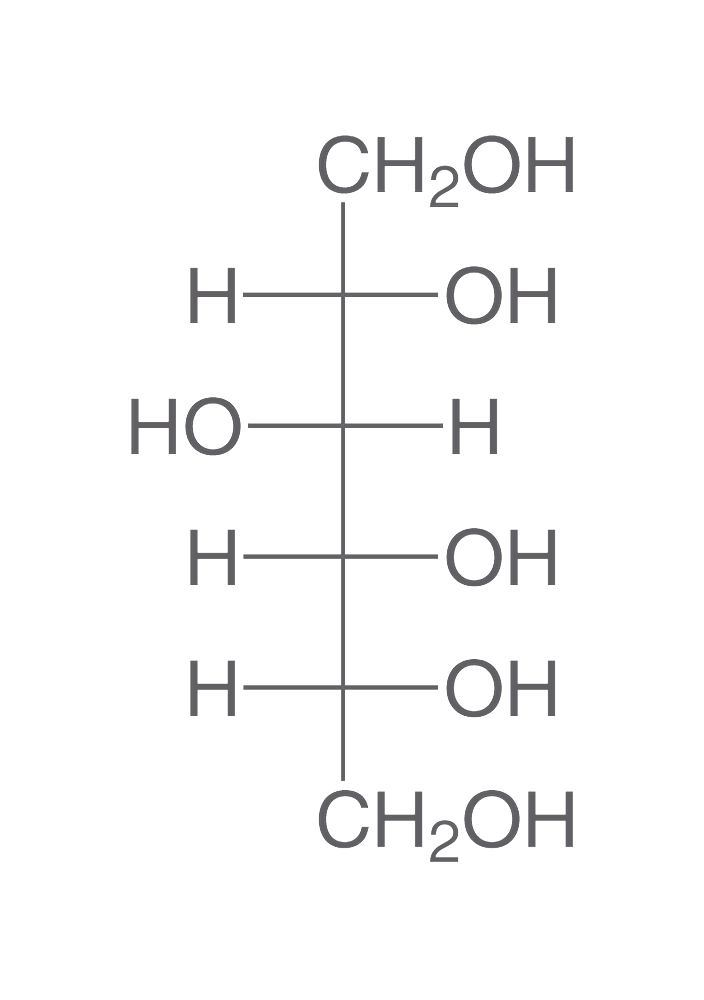
\includegraphics[width=0.12\textwidth]{sorbitol.jpeg}
  \end{wrapfigure}
  One alternative to sucrose, is \textbf{\textit{Sorbitol}}. Sorbitol is a sugar alcohol that has a higher melting point and different combustion characteristics compared to sucrose. By using sorbitol in the KNSu mixture, we can achieve a slower burn rate, which can be beneficial for pressure engines. A slower burn rate allows for a more controlled release of gases, resulting in a steadier thrust profile during the rocket's ascent. \\ 

  \vspace{-1cm}
  \begin{center}
    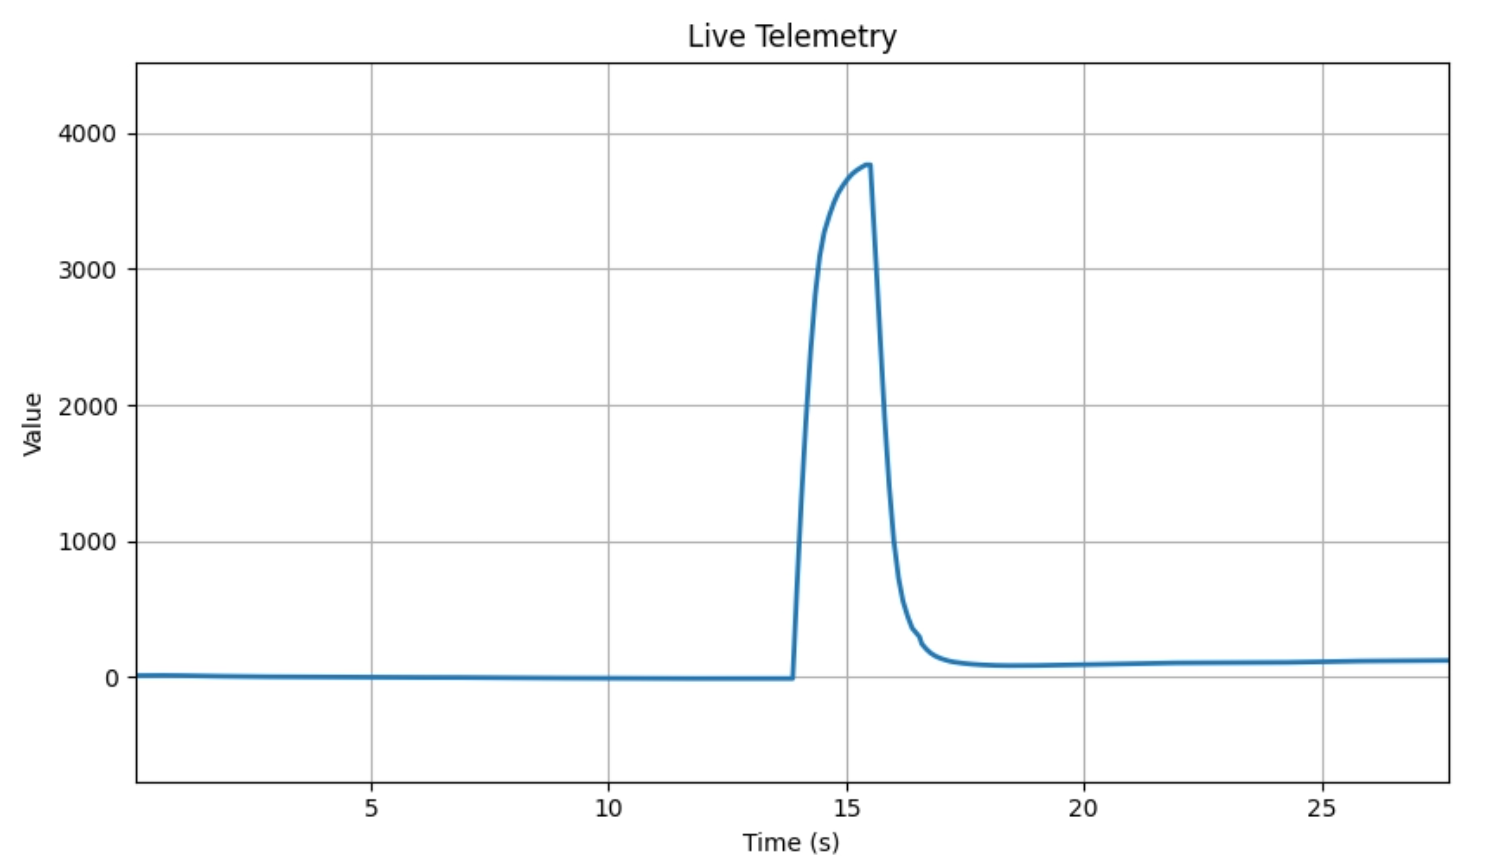
\includegraphics[width=0.5\textwidth]{sf_2.png}
  \end{center}

  We tested the motor using a sorbitol based grain this time, and the thrust was significantly more stronger. \\

   There is however another better way to improve thrust. The next modification would be altering the composition of Oxidizer. 
  \[ \boldsymbol{\underbrace{KNO_3}_{61 \%} \; + \; \underbrace{NH_4 NO_3}_{4 \%}} \] The only issue with this is the availability of ammonium nitrate. In India (like many parts of the world), there is a tight control over the supply of ammonium nitrate, owing to its notorious reputation of being used in explosives. We had to go for an alternative.
  

   
\end{multicols*}

  \newpage
  \begin{center}
    \textbf{\LARGE PHASE - II} \\
    \vspace{0.2cm}
    \textbf{\Large Recovery System Integration (Parachute + Ejection)}
  \end{center}

  \begin{multicols}{2}
      
  \addcontentsline{toc}{section}{\large 2. \textbf{PHASE - II :} Recovery System Integration (Parachute + Ejection)} 

  \noindent \textbf{\large OBJECTIVE:} \\ \textit{Integrate dual-deployment recovery system with ejection charge.} \\
  The main objective of this phase is to design and integrate a reliable recovery system for the model rocket, ensuring a safe and controlled descent after reaching apogee. The recovery system will consist of a parachute deployment mechanism triggered by an ejection charge, which will be activated at the appropriate altitude during the rocket's flight. This phase will involve careful consideration of the parachute sizing, ejection charge design, and deployment mechanism to ensure that the rocket can be safely recovered without damage. \\

  \noindent \textbf{DESIGN:}\\  \textit{Parachute sizing, ejection charge design, deployment mechanism.}\\ 
  The parachute will be sized based on the rocket's weight and descent rate, ensuring that it provides sufficient drag to slow the rocket's descent to a safe landing speed. The ejection charge will be designed to provide enough force to deploy the parachute effectively, without causing damage to the rocket or its components. The deployment mechanism will be carefully engineered to ensure reliable activation of the ejection charge at the desired altitude, using either a mechanical or electronic trigger system. \\

  \noindent \textbf{\large MATERIALS \& TOOLS:}\\  \textit{Nylon parachute, black powder ejection charge, altimeter (optional).}\\
  We are using a nylon parachute due to its durability and lightweight properties, which are essential for effective deployment and descent. The parachute will be custom-sized to match the rocket's weight and descent rate, ensuring optimal performance during recovery. The ejection charge will be constructed using black powder, a common choice for model rocketry due to its reliable ignition characteristics and sufficient thrust for parachute deployment. An altimeter may be included in the rocket's avionics package to provide accurate altitude data, allowing for precise timing of the ejection charge activation. This will help ensure that the parachute is deployed at the correct altitude, maximizing the chances of a safe and controlled landing. \\

  \noindent \textbf{\large TESTS:}\\  \textit{Deployment tests, ejection charge tests, drop tests.} \\
  Tests will be conducted to validate the deployment mechanism and ensure that the parachute deploys correctly when triggered by the ejection charge. This will involve a series of ground-based tests, including drop tests from a height to simulate the rocket's descent and verify that the parachute opens fully and provides adequate drag. Ejection charge tests will also be performed to confirm that the charge ignites reliably and generates sufficient force to deploy the parachute without damaging the rocket. These tests will help identify any potential issues with the recovery system and allow for adjustments to be made before the rocket is launched. \\

  \noindent \textbf{\large SUCCESS CRITERIA:}\\  \textit{Successful deployment of parachute at apogee, safe landing of rocket.} \\
  Success in this phase will be determined by the successful deployment of the parachute at apogee, resulting in a controlled and safe descent of the rocket. The parachute should fully open and provide sufficient drag to slow the rocket's descent to a safe landing speed, minimizing the risk of damage upon impact. The rocket should land intact, with all components, including the motor casing and recovery system, remaining undamaged and functional. Additionally, the deployment mechanism and ejection charge should operate reliably, with no failures or malfunctions during testing or actual flight. Meeting these criteria will demonstrate that the recovery system is effective and reliable, ensuring the safety of both the rocket and its surroundings during recovery operations. \\

  \noindent \textbf{\large RISKS \& MITIGATION:}\\  \textit{Ejection charge safety, parachute tangling, fire extinguisher.} \\
  We are taking the following risks and mitigation strategies into account for this phase: \\
n  \begin{itemize}
    \item Ejection charge safety: Proper handling and storage of the black powder ejection charge will be ensured, following all safety protocols to prevent accidental ignition. The charge will be kept in a secure container and only handled in a controlled environment. \\ 

      \item Parachute tangling: The parachute will be carefully packed and secured to prevent tangling during deployment. A deployment bag may be used to ensure that the parachute unfolds correctly when deployed. \\

        \item Fire extinguisher: A fire extinguisher will be kept on hand during all testing and launch activities to quickly address any potential fires that may arise from the ejection charge or other components. \\
  \end{itemize}
  
  \end{multicols}

  \section*{\Large IMPLEMENTATION FLOW:} 

  %==============================
% PHASE II : Recovery System Integration
%==============================
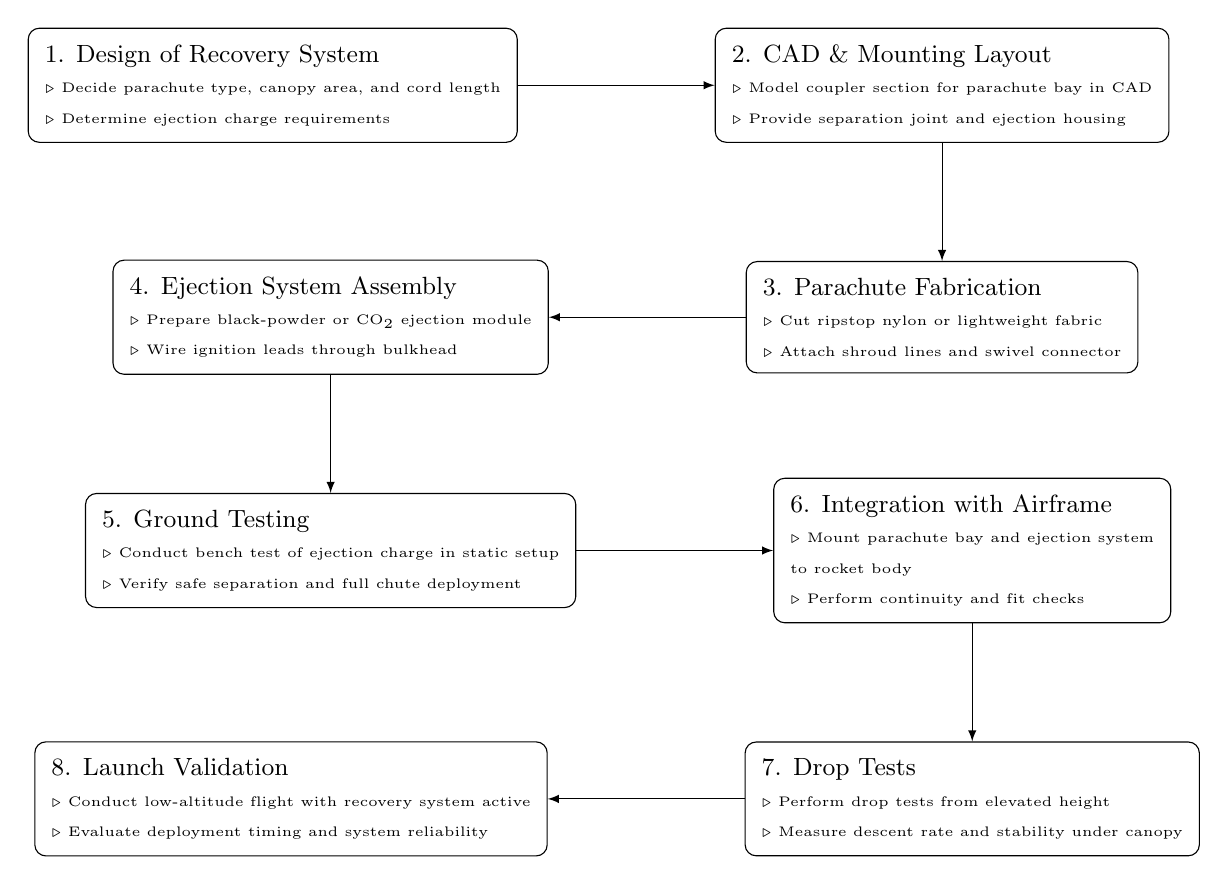
\begin{tikzpicture}[node distance=1.5cm and 2.5cm]

% Row 1 (→)
\node[box] (p2n1) at (0,0) {1. Design of Recovery System\\ 
\tiny$\triangleright$ Decide parachute type, canopy area, and cord length\\
\tiny$\triangleright$ Determine ejection charge requirements};
\node[box, right=of p2n1] (p2n2) {2. CAD \& Mounting Layout\\
\tiny $\triangleright$ Model coupler section for parachute bay in CAD\\
\tiny $\triangleright$ Provide separation joint and ejection housing};

% Row 2 (←)
\node[box, below=of p2n2] (p2n3) {3. Parachute Fabrication\\\tiny
$\triangleright$ Cut ripstop nylon or lightweight fabric\\\tiny
$\triangleright$ Attach shroud lines and swivel connector};
\node[box, left=of p2n3] (p2n4) {4. Ejection System Assembly\\\tiny
  $\triangleright$ Prepare black-powder or $\text{CO}_2$ ejection module\\\tiny
$\triangleright$ Wire ignition leads through bulkhead};

% Row 3 (→)
\node[box, below=of p2n4] (p2n5) {5. Ground Testing\\\tiny
$\triangleright$ Conduct bench test of ejection charge in static setup\\\tiny
$\triangleright$ Verify safe separation and full chute deployment};
\node[box, right=of p2n5] (p2n6) {6. Integration with Airframe\\\tiny
$\triangleright$ Mount parachute bay and ejection system \\\tiny to rocket body\\\tiny
$\triangleright$ Perform continuity and fit checks};

% Row 4 (←)
\node[box, below=of p2n6] (p2n7) {7. Drop Tests\\\tiny
$\triangleright$ Perform drop tests from elevated height\\\tiny
$\triangleright$ Measure descent rate and stability under canopy};
\node[box, left=of p2n7] (p2n8) {8. Launch Validation\\\tiny
$\triangleright$ Conduct low-altitude flight with recovery system active\\\tiny
$\triangleright$ Evaluate deployment timing and system reliability};

% ----- ARROWS -----
% Row1 →
\draw[arr] (p2n1.east) |- (p2n2.west);
% Down to row2 start
\draw[arr] (p2n2.south) -| (p2n3.north);
% Row2 ←
\draw[arr] (p2n3.west) |- (p2n4.east);
% Down to row3 start
\draw[arr] (p2n4.south) -| (p2n5.north);
% Row3 →
\draw[arr] (p2n5.east) |- (p2n6.west);
% Down to row4 end
\draw[arr] (p2n6.south) -| (p2n7.north);
% Row4 ←
\draw[arr] (p2n7.west) -- (p2n8.east);

\end{tikzpicture}

  \newpage
  \begin{center}
    \textbf{\LARGE PHASE - III} \\
    \vspace{0.2cm}
    \textbf{\Large Avionics \& Telemetry Deployment (GPS + Ground Station)}
  \end{center}
  \begin{multicols}{2}
      
  \addcontentsline{toc}{section}{\large 3. \textbf{PHASE - III :} Avionics \& Telemetry Deployment (GPS + Ground Station)}

  \noindent \textbf{\large OBJECTIVE:} \\ \textit{Incorporate GPS-based telemetry system for real-time flight data monitoring.} \\

  The main objective of this phase is to design and integrate an avionics system into the model rocket that includes a GPS-based telemetry system for real-time flight data monitoring. This system will provide valuable information about the rocket's position, altitude, speed, and other flight parameters during its ascent and descent. The telemetry data will be transmitted to a ground station, allowing for real-time monitoring and analysis of the rocket's performance. This phase will involve selecting appropriate components, designing the avionics package, and ensuring reliable communication between the rocket and the ground station. \\

  \noindent \textbf{\large DESIGN:}\\  \textit{GPS module, microcontroller, ground station setup.}\\
  For the GPS module, we are using the u-blox NEO-6M, which is a popular choice for model rocketry due to its compact size, low power consumption, and reliable performance. The microcontroller will be an Arduino Nano, which provides sufficient processing power and I/O capabilities for handling the GPS data and managing the telemetry transmission. The ground station setup will include a compatible RF receiver and software for displaying and analyzing the telemetry data in real-time. The overall design will focus on ensuring that the avionics package is lightweight, compact, and securely mounted within the rocket to withstand the stresses of launch and flight. \\

  \noindent \textbf{\large MATERIALS \& TOOLS:}\\  \textit{GPS module (e.g., u-blox NEO-6M), microcontroller (e.g., Arduino Nano), RF transmitter/receiver, ground station software (e.g., Mission Planner).}\\
  As mentioned earlier, the GPS module will be the u-blox NEO-6M, which provides accurate positioning data and is widely used in model rocketry applications. The microcontroller will be an Arduino Nano, which is a compact and versatile platform for handling the GPS data and managing the telemetry transmission. The RF transmitter/receiver pair will be selected based on the desired range and data rate, ensuring reliable communication between the rocket and the ground station. The ground station software will be Mission Planner, which is a popular choice for displaying and analyzing telemetry data in real-time. This software provides a user-friendly interface and supports various telemetry protocols, making it suitable for our application. \\

  \noindent \textbf{\large TESTS:}\\  \textit{Bench tests, range tests, integration tests.}\\
  Tests will be conducted to validate the functionality and reliability of the avionics and telemetry system. Bench tests will be performed to verify that the GPS module is providing accurate position data and that the microcontroller is correctly processing and transmitting this data. Range tests will be conducted to ensure that the RF transmitter/receiver pair can maintain a reliable communication link over the expected distance between the rocket and the ground station. Integration tests will be performed to confirm that all components of the avionics package are working together seamlessly, with successful data transmission and reception during simulated flight conditions. These tests will help identify any potential issues with the avionics system and allow for adjustments to be made before the rocket is launched. \\

  \noindent \textbf{\large SUCCESS CRITERIA:}\\  \textit{Accurate real-time telemetry data, successful ground station communication.}\\
  This phase will be considered successful if the avionics and telemetry system provides accurate real-time data during flight, including position, altitude, speed, and other relevant parameters. The GPS module should demonstrate reliable performance, with minimal signal loss or inaccuracies in the position data. The microcontroller should effectively process and transmit the telemetry data to the ground station, with successful communication established between the rocket and the ground station throughout the flight. The ground station software should be able to display and analyze the telemetry data in real-time, providing valuable insights into the rocket's performance. Meeting these criteria will demonstrate that the avionics and telemetry system is effective and reliable, enhancing the overall capabilities of the model rocket. \\

  \noindent \textbf{\large RISKS \& MITIGATION:}\\  \textit{Signal interference, power management, secure mounting.}\\
  The risks and mitigation strategies for this phase include: \\
  \begin{itemize}
    \item Signal interference: The RF communication link may be subject to interference from other electronic devices or environmental factors. To mitigate this risk, we will select a frequency band that is less congested and use shielding techniques to minimize interference. \\

      \item Power management: The avionics system will require a reliable power source to ensure continuous operation during flight. We will use a high-capacity lithium polymer (LiPo) battery and implement power management strategies to optimize battery life and prevent power loss during critical flight phases. \\

        \item Secure mounting: The avionics components must be securely mounted within the rocket to withstand the stresses of launch and flight. We will use vibration-damping materials and secure mounting techniques to protect the components from damage and ensure reliable operation throughout the flight. \\
  \end{itemize}

%==============================
% PHASE III : Avionics & Telemetry Deployment
%==============================
  %


\end{multicols}  
\noindent \textbf{IMPLEMENTATION FLOW:} \\
\vspace{0.5cm}

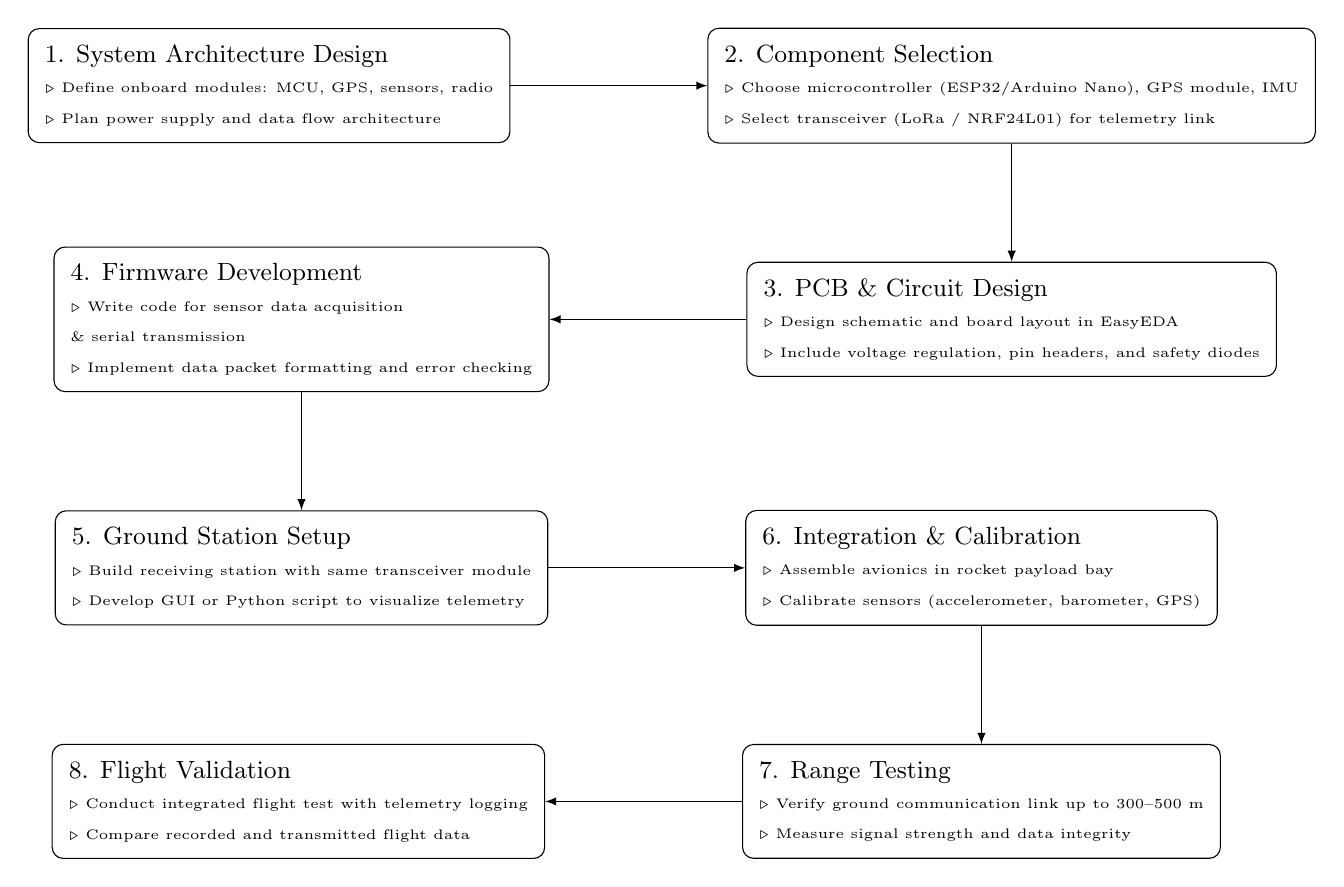
\begin{tikzpicture}[node distance=1.5cm and 2.5cm]
% Row 1 (→)
\node[box] (p3n1) at (0,0) {1. System Architecture Design\\\tiny
$\triangleright$ Define onboard modules: MCU, GPS, sensors, radio\\\tiny
$\triangleright$ Plan power supply and data flow architecture};
\node[box, right=of p3n1] (p3n2) {2. Component Selection\\\tiny
$\triangleright$ Choose microcontroller (ESP32/Arduino Nano), GPS module, IMU\\\tiny
$\triangleright$ Select transceiver (LoRa / NRF24L01) for telemetry link};

% Row 2 (←)
\node[box, below=of p3n2] (p3n3) {3. PCB \& Circuit Design\\\tiny
$\triangleright$ Design schematic and board layout in EasyEDA\\\tiny
$\triangleright$ Include voltage regulation, pin headers, and safety diodes};
\node[box, left=of p3n3] (p3n4) {4. Firmware Development\\\tiny
  $\triangleright$ Write code for sensor data acquisition \\\tiny \& serial transmission\\\tiny
$\triangleright$ Implement data packet formatting and error checking};

% Row 3 (→)
\node[box, below=of p3n4] (p3n5) {5. Ground Station Setup\\\tiny
$\triangleright$ Build receiving station with same transceiver module\\\tiny
$\triangleright$ Develop GUI or Python script to visualize telemetry};
\node[box, right=of p3n5] (p3n6) {6. Integration \& Calibration\\\tiny
$\triangleright$ Assemble avionics in rocket payload bay\\\tiny
$\triangleright$ Calibrate sensors (accelerometer, barometer, GPS)};

% Row 4 (←)
\node[box, below=of p3n6] (p3n7) {7. Range Testing\\\tiny
$\triangleright$ Verify ground communication link up to 300–500 m\\\tiny
$\triangleright$ Measure signal strength and data integrity};
\node[box, left=of p3n7] (p3n8) {8. Flight Validation\\\tiny
$\triangleright$ Conduct integrated flight test with telemetry logging\\\tiny
$\triangleright$ Compare recorded and transmitted flight data};

% ----- ARROWS -----
% Row1 →
\draw[arr] (p3n1.east) |- (p3n2.west);
% Down to row2 start
\draw[arr] (p3n2.south) -| (p3n3.north);
% Row2 ←
\draw[arr] (p3n3.west) |- (p3n4.east);
% Down to row3 start
\draw[arr] (p3n4.south) -| (p3n5.north);
% Row3 →
\draw[arr] (p3n5.east) |- (p3n6.west);
% Down to row4 end
\draw[arr] (p3n6.south) -| (p3n7.north);
% Row4 ←
\draw[arr] (p3n7.west) |- (p3n8.east);

\end{tikzpicture}

  \newpage 
  \begin{center}
    \textbf{\LARGE PHASE - IV} \\
    \vspace{0.2cm}
    \textbf{\Large Thrust Vector Control Implementation (Nozzle Steering)}
  \end{center}
  \begin{multicols}{2}
  \addcontentsline{toc}{section}{\large 4. \textbf{PHASE - IV :} Thrust Vector Control Implementation (Nozzle Steering)}

  \noindent \textbf{\large OBJECTIVE:} \\ \textit{Implement thrust vector control (TVC) for enhanced flight stability and maneuverability.} \\
  Objective of this phase is to design and implement a thrust vector control (TVC) system for the model rocket, which will enhance its flight stability and maneuverability. The TVC system will allow for active control of the rocket's trajectory by adjusting the direction of the thrust produced by the motor. This will enable the rocket to maintain a stable flight path, compensate for external disturbances such as wind, and perform controlled maneuvers during ascent. The implementation of TVC will involve selecting appropriate actuators, designing control algorithms, and integrating the system with the existing avionics package. \\

  \noindent \textbf{\large DESIGN:}\\  \textit{TVC mechanism, servo motors, control algorithms.}\\
  The main component of the TVC system will be the nozzle steering mechanism, which will be designed to allow for precise adjustments to the direction of the thrust vector. This will involve the use of servo motors, such as MG90S, which are capable of providing the necessary torque and speed for effective nozzle movement. The servo motors will be controlled by a microcontroller, such as an Arduino Nano, which will execute control algorithms to determine the appropriate nozzle position based on flight data from the avionics package. The control algorithms will be designed to respond to changes in flight conditions, such as deviations from the desired trajectory or external disturbances, and adjust the nozzle position accordingly to maintain stability and control. \\

  \noindent \textbf{\large MATERIALS \& TOOLS:}\\  \textit{Servo motors (e.g., MG90S), microcontroller (e.g., Arduino Nano), IMU sensor (e.g., MPU6050).}\\
  To achieve thrust vector control, we will use MG90S servo motors, which are known for their reliability and performance in model rocketry applications. These servo motors will be integrated into the nozzle steering mechanism, allowing for precise adjustments to the thrust vector during flight. The microcontroller will be an Arduino Nano, which will handle the control algorithms and manage the servo motor movements based on input from the avionics package. An IMU sensor, such as the MPU6050, will be included in the avionics package to provide real-time data on the rocket's orientation and acceleration. This data will be used by the control algorithms to determine the necessary adjustments to the nozzle position for maintaining stability and control during flight. \\

  \noindent \textbf{\large TESTS:}\\  \textit{Static tests, flight tests, control response tests.}\\
  Tests will be conducted to validate the functionality and performance of the thrust vector control system. Static tests will be performed to verify that the servo motors can effectively adjust the nozzle position and that the control algorithms are functioning as intended. These tests will involve simulating various flight conditions and observing the response of the TVC system to ensure that it can maintain stability and control. Flight tests will be conducted to evaluate the performance of the TVC system in real-world conditions, assessing its ability to compensate for external disturbances and maintain a stable trajectory during ascent. Control response tests will be performed to measure the responsiveness of the TVC system, ensuring that it can make rapid adjustments to the nozzle position as needed to maintain stability and control throughout the flight. \\

  \noindent \textbf{\large SUCCESS CRITERIA:}\\  \textit{Improved flight stability, successful maneuvering during flight.}\\
  This will be considered successful if the thrust vector control system demonstrates improved flight stability and the ability to perform controlled maneuvers during flight. The TVC system should effectively compensate for external disturbances, such as wind or turbulence, maintaining a stable trajectory throughout the ascent. The servo motors should respond quickly and accurately to control inputs, allowing for precise adjustments to the nozzle position as needed. Additionally, the integration of the TVC system with the existing avionics package should be seamless, with reliable communication and coordination between the components. Meeting these criteria will demonstrate that the thrust vector control system is effective and enhances the overall performance of the model rocket. \\

  \noindent \textbf{\large RISKS \& MITIGATION:}\\  \textit{Mechanical failure, power consumption, secure mounting.}\\
  Risks and mitigation strategies for this phase include: \\
  \begin{itemize}
    \item Mechanical failure: The servo motors and nozzle steering mechanism may be subject to mechanical failure due to the stresses of launch and flight. To mitigate this risk, we will use high-quality components and implement robust mounting techniques to ensure that the system can withstand the forces experienced during flight. \\

      \item Power consumption: The TVC system will require additional power to operate the servo motors, which may impact the overall power budget of the rocket. We will carefully manage power consumption by optimizing the control algorithms and using efficient components to minimize the impact on battery life. \\

        \item Secure mounting: The TVC components must be securely mounted within the rocket to prevent damage or dislodging during flight. We will use vibration-damping materials and secure mounting techniques to protect the components and ensure reliable operation throughout the flight. \\
  \end{itemize}
  
  \end{multicols}

  \noindent \textbf{IMPLEMENTATION FLOW:} \\
  \vspace{0.5cm}

  %==============================
% PHASE IV : Thrust Vector Control Implementation
%==============================
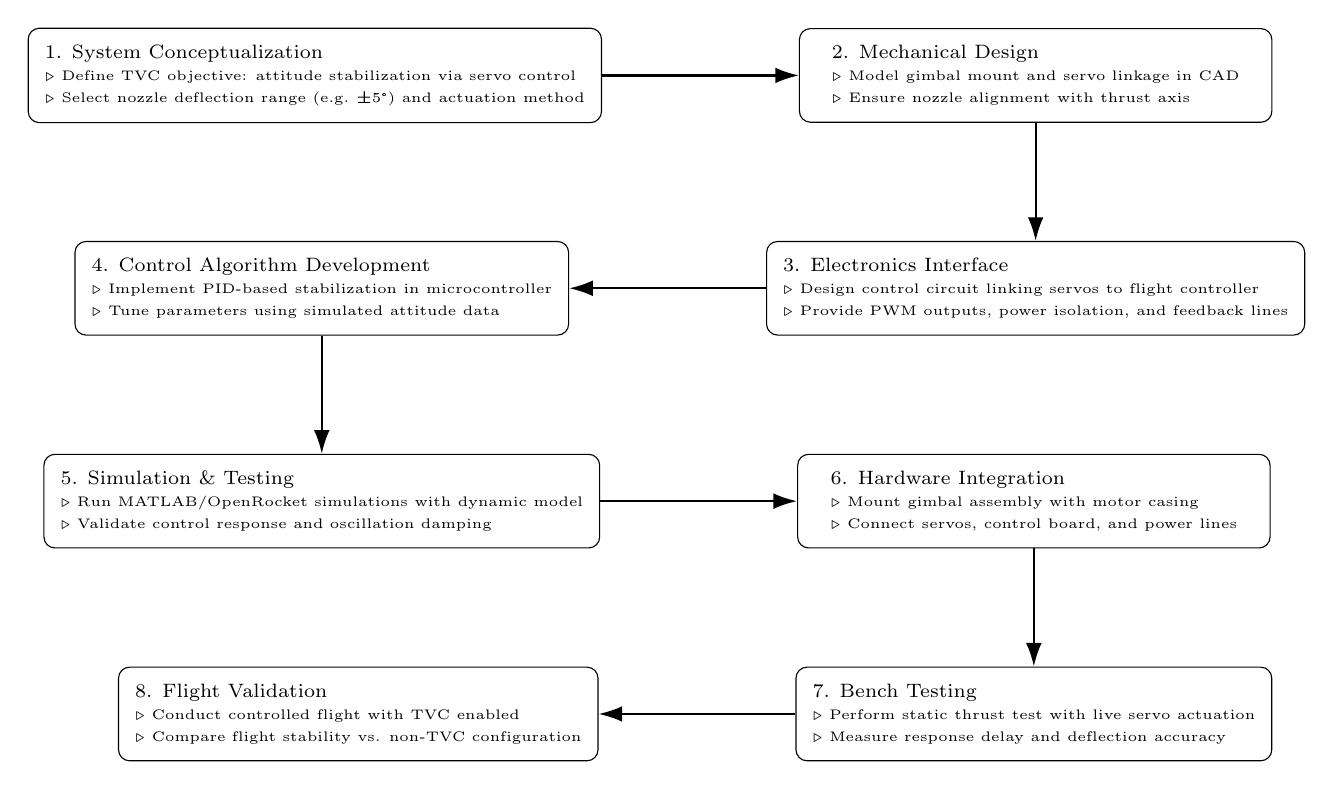
\begin{tikzpicture}[node distance=1.5cm and 2.5cm]
\tikzset{
  box/.style = {rectangle, draw=black, rounded corners,
                minimum width=6cm, minimum height=1.1cm,
                align=left, font=\scriptsize, inner sep=6pt},
  arr/.style = {-{Latex[length=3mm,width=2mm]}, line width=0.8pt}
}

% Row 1 (→)
\node[box] (p4n1) at (0,0) {1. System Conceptualization\\\tiny
$\triangleright$ Define TVC objective: attitude stabilization via servo control\\\tiny
$\triangleright$ Select nozzle deflection range (e.g. ±5°) and actuation method};
\node[box, right=of p4n1] (p4n2) {2. Mechanical Design\\\tiny
$\triangleright$ Model gimbal mount and servo linkage in CAD\\\tiny
$\triangleright$ Ensure nozzle alignment with thrust axis};

% Row 2 (←)
\node[box, below=of p4n2] (p4n3) {3. Electronics Interface\\\tiny
$\triangleright$ Design control circuit linking servos to flight controller\\\tiny
$\triangleright$ Provide PWM outputs, power isolation, and feedback lines};
\node[box, left=of p4n3] (p4n4) {4. Control Algorithm Development\\\tiny
$\triangleright$ Implement PID-based stabilization in microcontroller\\\tiny
$\triangleright$ Tune parameters using simulated attitude data};

% Row 3 (→)
\node[box, below=of p4n4] (p4n5) {5. Simulation \& Testing\\\tiny
$\triangleright$ Run MATLAB/OpenRocket simulations with dynamic model\\\tiny
$\triangleright$ Validate control response and oscillation damping};
\node[box, right=of p4n5] (p4n6) {6. Hardware Integration\\\tiny
$\triangleright$ Mount gimbal assembly with motor casing\\\tiny
$\triangleright$ Connect servos, control board, and power lines};

% Row 4 (←)
\node[box, below=of p4n6] (p4n7) {7. Bench Testing\\\tiny
$\triangleright$ Perform static thrust test with live servo actuation\\\tiny
$\triangleright$ Measure response delay and deflection accuracy};
\node[box, left=of p4n7] (p4n8) {8. Flight Validation\\\tiny
$\triangleright$ Conduct controlled flight with TVC enabled\\\tiny
$\triangleright$ Compare flight stability vs. non-TVC configuration};

% ----- ARROWS -----
% Row1 →
\draw[arr] (p4n1.east) |- (p4n2.west);
% Down to row2 start
\draw[arr] (p4n2.south) -| (p4n3.north);
% Row2 ←
\draw[arr] (p4n3.west) |- (p4n4.east);
% Down to row3 start
\draw[arr] (p4n4.south) -| (p4n5.north);
% Row3 →
\draw[arr] (p4n5.east) |- (p4n6.west);
% Down to row4 end
\draw[arr] (p4n6.south) -| (p4n7.north);
% Row4 ←
\draw[arr] (p4n7.west) |- (p4n8.east);

\end{tikzpicture}

\end{document}
